\documentclass[12pt, letterpaper]{article}
\usepackage[utf8]{inputenc}
\usepackage{cite}
\usepackage{float}
\usepackage{tikz}
\usepackage{hyperref}
\usepackage[newfloat]{minted}
\usepackage{caption}
\usepackage{dirtree}
\tolerance=1
\emergencystretch=\maxdimen
\hyphenpenalty=10000
\hbadness=10000

\newenvironment{code}{\captionsetup{type=listing}}{}
\SetupFloatingEnvironment{listing}{name=Source Code}

\graphicspath{{images/}}

\title{Einfacher Redis-Client mit RESP3\\Beispiel 33}
\author{Marcel Dinhof, 5BHIF\\Katalognummer: 3}
\date{April 2022}

\begin{document}

\begin{titlepage}
\maketitle
\end{titlepage}

\tableofcontents
\newpage

\section{Einleitung}
Das Ziel dieses Projektes ist die Umsetzung eines einfachen, auf dem Protokoll RESP3 basierenden, Redis-Clients. Dieser soll Funktionalitäten wie Pipelining, Publishing/Subscribing, Transaktionen, als auch verteilte Locks implementieren.

\section{RESP3}\label{sec:RESP3}
RESP3 ist ein Protokoll für die Kommunikation zwischen einem Redis-Client und einem Redis Server.
In der folgenden Auflistung werden grundlegende Datentypen des RESP3 Protokolls dargestellt. Aus Gründen der Lesbarkeit werden die Zeichen "{{\textbackslash}r}{{\textbackslash}n}" durch {$<$CR$>$}{$<$LF$>$} dargestellt.

\begin{figure}[h]
\begin{verbatim}
+---------------+------------------------------------------+
| Datentyp      | RESP Darstellung                         | 
+---------------+------------------------------------------+
| Simple String | +MSG<CR><LF>                             | 
+---------------+------------------------------------------+
| Bulk String   | $MSG-SIZE<CR><LF>MSG<CR><LF>             |
+---------------+------------------------------------------+
| Integer       | :MSG<CR><LF>                             |
+---------------+------------------------------------------+
| Error         | -MSG<CR><LF>                             |
+---------------+------------------------------------------+
| Array         | *ARRAY-SIZE<CR><LF>ELEMENTS<CR><LF>      |
+---------------+------------------------------------------+
| Map           | %MAP-SIZE<CR><LF>KEY/VALUE-PAIRS<CR><LF> |
+---------------+------------------------------------------+
\end{verbatim}
\caption{Liste der in diesem Projekt benutzten Redis-Datentypen mit ihrem Aufbau}
\end{figure}

\section{Funktionalitäten}
\subsection{Pipelining}
\textit{Pipelining}\cite{pipelining} ist eine Taktik zur Netzwerk-Optimierung, bei der Befehle nicht sofort zum Server gesendet, sondern beim Client gepuffert werden. Dieser sendet zu einem späteren Zeitpunkt alle Anweisungen gleichzeitig an den Server. Pipelining ist nicht mit Transaktionen (Sektion \ref{sec:transaktionen}) zu verwechseln, da keine Garantie für die Ausführung der Befehle gewährleistet wird.

\subsection{Publish und Subscribe}
Die Befehle \textit{Publish} und \textit{Subscribe} können genutzt werden, um Nachrichten an alle Clients zu senden, die einen bestimmten Wert mittels Subscribe überwachen\cite{subpub}. 

\subsection{Transaktionen}\label{sec:transaktionen}
Eine weitere Funktionalität von Redis ist die Nutzung von \textit{Transaktionen}\cite{transaktion}. Transaktionen ermöglichen die gleichzeitige Ausführung von mehreren Befehlen, die als eine Einheit sequenziell abgearbeitet werden\cite{transaktion}.
Die Kommandos für Transaktionen sind:
\begin{itemize}
    \item \textit{MULIT} - Startet eine Transaktion.
    \item \textit{EXEC} - Führt eine Transaktion aus und beendet diese.
    \item \textit{DISCARD} - Verwirft die gesammelten Befehle und beendet eine Transaktion.
\end{itemize}

\subsection{Redlock}
\textit{Redlocks}\cite{redlock} bieten die Möglichkeit, Sperren in einem Verbund an Redis-Clients anzufordern. Dabei wird einem Schlüsselelement ein zufällig generierter Wert zugewiesen. Wenn die Sperre angefordert wird, versucht der Client diesen Schlüssel mit seinem eindeutigen Wert zu setzen. Sollte dieser schon von einem anderen Client gesetzt worden sein, wartet der Client darauf, dass der Schlüssel am Server entfernt wird und er seinen eigenem Wert setzen darf. Beim Entsperren wird der Wert von Redis mit dem lokalen Wert des Clients abgeglichen. Nur wenn diese identisch sind, darf die Sperre aufgehoben werden.

\section{Struktur}

\subsection{Konventionen}
Für Klassennamen wurde in diesem Projekt "Pascal case" und für Funktionsnamen sowie für Variablennamen "Snake case" verwendet. Verwendete Bibliotheken werden in Sektion \ref{sec:biblio} zusammengefasst und grundlegend beschrieben.

\subsection{Klassendiagramm}
\begin{figure}[H]
  \centering
  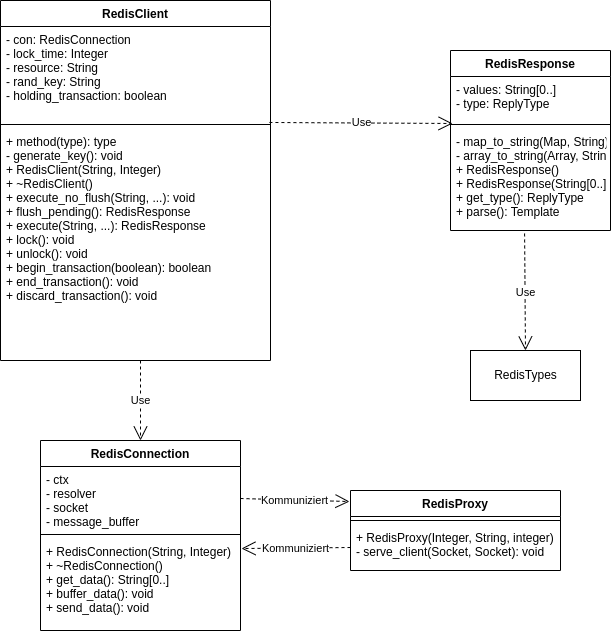
\includegraphics[width=.7\textwidth]{klassendiagram.png}
  \caption{Klassendiagramm}
  \label{fig:kdg}
\end{figure}

\subsection{RedisClient}
Die Klasse RedisClient implementiert alle Funktionalitäten, die der Client zur Verfügung stellt.

\subsection{RedisConnection}
Die Klasse RedisConnection implementiert die Funktionen für eine Kommunikation mit einem Redis Server. Die Klasse verfügt über Methoden zum Lesen, Schreiben und Puffern der Daten. 

\subsection{RedisType Klassen}
Für die Serialisierung und Speicherung der Rückgabewerte eines Redis-Servers wurden für jeden, in Sektion \ref{sec:RESP3} beschriebenen, RESP3 Datentypen eine eigene Klasse implementiert.
Dem Konstruktor dieser Klassen wird eine \textit{deque} mit \textit{strings} übergeben, deren Inhalt in die entsprechende Datenstruktur (z.B. SimpleString, BulkString, ...) überführt wird.

\subsection{RedisResponse}
Die RedisResponse Klasse implementiert einen Konstruktor, der den Typen eines empfangenen Rückgabewertes aus dem ersten Teil der Nachricht verarbeitet. Des Weiteren sind in der Klasse überladene \textit{parse} - Methoden implementiert. Beim Aufruf einer \textit{parse} - Methode muss ein Datentyp für die Rückgabe angegeben werden. Daraufhin wird versucht, die empfangene Nachricht in diesen Typen zu überführen, beispielsweise durch Konvertierung eines \textit{integer} in einen \textit{string}. Folgende Datentypen können für die Rückgabe ausgewählt werden: 
\begin{itemize}
    \item \textit{string}
    \item \textit{integer}
    \item \textit{Redis::Array}
    \item \textit{Redis::Map}
\end{itemize}
Sollte ein RedisType nicht in den spezifizierten Datentypen geparsed werden können, löst die Funktion eine Ausnahme aus.

\subsection{RedisProxy}
Implementiert einen Proxy-Server, der einerseits mittels Protobuf (beschrieben in Sektion \ref{sec:proto}) mit einem Redis-Client kommuniziert und dessen Nachrichten an einen Redis-Server weiterleitet, und andererseits die Nachrichten von einem Redis-Server in Protobuf überführt und an einen Client sendet.

\subsection{Logger}
In der Datei logger.h wird das Logging mit \textit{spdlog} über Präprozessoranweisungen implementiert. Der Detaillierungsgrad des Loggens kann durch \textit{SET\_LOGLEVEL} angepasst werden.

\section{Redis Befehle}
In diesem Abschnitt werden Kommandos vorgestellt, die in diesem Client genutzt wurden um die geforderten Funktionalitäten zu implementieren. Eine vollständige Dokumentation zu allen Redis-Befehlen kann auf der offiziellen Website\cite{redis_commands} nachgelesen werden.

\paragraph{SET [key] [value]}
Speichert einen angegebenen Wert mit einem eindeutigen Schlüssel.

\paragraph{SET [key] [value] NX}
NX gibt an, dass der Wert nur gesetzt wird, wenn er noch nicht existiert.

\paragraph{SET [key] [value] PX [time]}
Die Option PX kann benutzt werden, um ein Element nach einer angegebenen Zeit (in Millisekunden) zu löschen.

\paragraph{GET [key]}
Liefert den Wert zurück, der mit dem angegebenen Schlüssel gespeichert wurde. Falls kein Wert vorhanden ist, ist der Rückgabewert null.

\paragraph{MULTI}
Der MULTI Befehl wird genutzt, um Transaktionen zu starten.

\paragraph{DISCARD}
Transaktionen können mit DISCARD abgebrochen werden.

\paragraph{EXEC}
Transaktionen können mit EXEC ausgeführt werden.


\section{Implementierungsbeispiele}
\subsection{Parsen in einen Redis Datentypen}

\subsubsection{SimpleString Klasse}
Im Konstruktor der \textit{RedisType} Klassen werden die empfangenen Nachrichten entsprechend angepasst. Da ein \textit{SimpleString} mit einem '+' beginnt, wird dieses Zeichen entfernt.

\begin{code}
\begin{minted}{cpp}
class SimpleString {
private:
    std::string content{};
public:
    SimpleString(std::deque<std::string>& msg) {
        content = msg.at(0);
        msg.pop_front();
    }

    std::string& get() {
        return content;
    }
};
\end{minted}
\caption{SimpleString Klasse}
\label{resolve_domain}
\end{code}

\subsubsection{Array Parsing}
Sowohl ein Array als auch eine \textit{Map} können alle, in Sektion \ref{sec:RESP3} beschriebenen, Datentypen beinhalten. Aus diesem Grund wird bei jeder Einfügeoperation der Typ der empfangenen Nachricht ermittelt, und dementsprechend wird die dazugehörige Klasse erzeugt.

\begin{code}
\begin{minted}{cpp}
switch (determin_type(msg.at(0))) {
    case ReplyType::simple_string:
        content.push_front(std::make_shared<redis_types>(SimpleString(msg)));
        break;
    case ReplyType::bulk_string:
        content.push_front(std::make_shared<redis_types>(BulkString(msg)));
        break;
    case ReplyType::integer:
        content.push_front(std::make_shared<redis_types>(Integer(msg)));
        break;  
    case ReplyType::error:
        content.push_front(std::make_shared<redis_types>(Error(msg)));
        break;  
    case ReplyType::array:
        content.push_front(std::make_shared<redis_types>(Array(msg)));
        break;  
    default:
        break;
    }
}
\end{minted}
\caption{Parsen eines Redis Arrays}
\label{resolve_domain}
\end{code}


\subsection{Ausführung von Befehlen}
Methoden zur Ausführung von Befehlen sind in der RedisClient Klasse implementiert. Es wird zwischen den beiden Methoden \textit{execute\_no\_flush} und \textit{execute} unterschieden.
\subsubsection{execute no flush}
Die execute\_no\_flush Methode wird in der execute Methode aufgerufen. Nach dem Parameteroperation können beliebig viele weitere Argumente übergeben werden. Ist die Verbindung zum Redis-Server aktiv, werden die übergebenen Werte in einen RESP3 konformen string überführt. Die daraus resultierende Zeichenkette wird an den Server gesendet.

\begin{code}
\begin{minted}{cpp}
template<typename ...T>
void execute_no_flush(std::string operation, T ... args) {
    if (con == nullptr) {
        LOG_ERROR("No connection!");
        return;
    } 
    std::deque<std::string> cmd {
        "$" + std::to_string(operation.length()) +
        operation,
        (
            "$" + std::to_string(std::string{args}.length()) +
            std::string{args}
        ) ...
    };
    cmd.push_front("*" + std::to_string(cmd.size()));
    RESP3Request request;
    for (const auto& e : cmd) {
        request.add_argument(e);
    }
    con->bufferData(request);
}
\end{minted}
\caption{execute\_no\_flush Methode aus der RedisClient Klasse.}
\label{resolve_domain}
\end{code}

\subsubsection{execute}
Die Parameter der execute Methode werden der execute\_no\_flush Methode übergeben, und danach wird der Puffer der Verbindungs-Klasse geleert.
Der Rückgabewert der Methode ist ein RedisResponse Objekt, dem die empfangenen Daten im Konstruktor übergeben werden.

\begin{code}
\begin{minted}{cpp}
template<typename ...T>
RedisResponse execute(std::string operation, T && ... args) {
    if (con == nullptr) {
        LOG_ERROR("No connection!");
        return RedisResponse{};
    } 
    execute_no_flush(operation, args...);
    con->sendData();
    return RedisResponse{con->getData()};
}
\end{minted}
\caption{execute Methode aus der RedisClient Klasse.}
\label{resolve_domain}
\end{code}

\subsection{Protocol buffers}\label{sec:proto}
\textit{Protobuf}\cite{protobuf} ist Plattformunabhängig und kann in Kombination mit unterschiedlichen Programmiersprachen verwendet werden, um strukturierte Daten zu serialisieren. Die Struktur der Daten wird in einer \textit{.proto} Datei festgelegt, deren Elemente sog. \textit{Messages} sind. Folgende Struktur wurde für diesen Redis-Client implementiert.
\begin{code}
\begin{minted}{text}
syntax = "proto3";

message Message {
    repeated string argument = 1;
}

message MessageBundle {
    string mode = 1;
    repeated Message message = 2;
}
\end{minted}
\end{code}
RESP3Responses werden zum Serialisieren der Daten verwendet, die vom Server gesendet wurden. RESP3Commands werden zum Serialisieren der Kommandos verwendet, die zum Server gesendet werden.

\section{Verwendete Bibliotheken}
\label{sec:biblio}

\subsection{CLI11}
\textit{CLI11}\cite{cli11} kann zum Verarbeiten von Kommandozeilenparametern verwendet werden und bietet unter anderem Möglichkeiten zur Implementierung von Interfaces und für die Validierung von Eingaben.

\subsection{spdlog}
Spdlog ist eine header-only Bibliothek zur Erstellung von Logging Ausgaben in einem Programm.

\section{Verwendung des Clients}
\label{usage}

\subsection{Kommandozeilenargumente}

\paragraph{--ip}
Die IP-Addresse des Redis-Servers, mit dem der Client eine Verbindung aufbauen soll.

\paragraph{-p,--port}
Der Port des Redis-Servers, mit dem der Client eine Verbindung aufbauen soll.


\begin{code}
  \begin{minted}{text}
./redis_client -h

A simple redis client
Usage: ./redis_client [OPTIONS]

Options:
  -h,--help                   Print this help message and exit
  --ip TEXT                   ip address to connect to
  -p,--port INT               port to connect to
  \end{minted}
  \caption{Ausgabe der Hilfestellung des Clients}
\end{code}

\subsection{Beispiele}
Folgende Beispiele veranschaulichen, wie dieser Client zu benutzen ist. In den Beispielen wird davon ausgegangen, dass jeder Rückgabewert zu einer Zeichenkette konvertierbar ist. 

\newpage

\subsubsection{SET und GET}
\begin{code}
\begin{minted}{cpp}
Redis::RedisClient client{ip_address, destination_port};
if (!client.is_connected()) {
    //error handling
    return 1;
}
std::string output;
output = client.execute("SET", "name", "MaxMuster123").parse<std::string>();
LOG_INFO(output);
output = client.execute("GET", "name").parse<std::string>();
LOG_INFO(output);

>> +OK
>> MaxMuster123
\end{minted}  
\end{code}

\subsubsection{Pipelining}
\begin{code}
\begin{minted}{cpp}
client.execute_no_flush("SET", "name", "MaxMuster321");
client.execute_no_flush("GET", "name");
std::vector<Redis::RedisResponse> responses{client.flush_pending()};
for (Redis::RedisResponse& response : responses) {
    LOG_INFO(response.parse<std::string>() << std::endl);
}

>> +OK
>> MaxMuster123
\end{minted}  
\end{code}



\subsubsection{Transaktionen}
\begin{code}
\begin{minted}{cpp}
output = client.execute("SET", "name", "MaxMuster321").parse<std::string>();
LOG_INFO(output);
client.begin_transaction();
output = client.execute("SET", "name", "MaxMuster123").parse<std::string>();
LOG_INFO(output);
output = client.execute("GET", "name").parse<std::string>();
LOG_INFO(output);
//client.end_transaction();      -> Transaktion wird durchgeführt
client.discard_transaction(); // -> Transaktion wird abgebrochen
output = client.execute("GET", "name").parse<std::string>();
LOG_INFO(output);
    
>> +QUEUED
>> +QUEUED
>> +OK
>> MaxMuster321
\end{minted}  
\end{code}

\subsubsection{Redlock}
\begin{code}
\begin{minted}{cpp}

client.lock("resource_1");
output = client.execute("SET", "name", "MaxMuster123").parse<std::string>();
LOG_INFO(output);
output = client.execute("GET", "name").parse<std::string>();
LOG_INFO(output);
client.unlock("resource_1");

>> +OK
>> MaxMuster123
\end{minted}  
\end{code}

\subsubsection{Subscribe}
\begin{code}
\begin{minted}{cpp}

client.subscribe("subscribe_object");
while (true) {
    LOG_INFO("Subscriber waiting for data");
        
    std::vector<Redis::RedisResponse> responses{client.fetch_data()};
    for (Redis::RedisResponse& response : responses) {
        LOG_INFO(response.parse<std::string>());
    }
}

>> ...
\end{minted}  
\end{code}

\subsubsection{Publish}
\begin{code}
\begin{minted}{cpp}
std::string input{};
while (true) {
    std::cout << "Element: ";
    std::getline(std::cin, input);
    output = client.execute("PUBLISH", "subscribe_object", input).parse<std::string>();
    LOG_INFO(output);
}

>> ...
\end{minted}  
\end{code}

\newpage

\section{Projektstruktur}
\dirtree{%
  .1 /.
  .2 LICENSE.
  .2 meson\_options.txt.
  .2 meson.build.
  .2 README.md.
  .2 CHANGELOG.org.
  .2 .gitignore.
  .2 include.
  .3 logger.h.
  .3 proxy.hpp.
  .3 redis\_client.hpp.
  .3 redis\_connection.hpp.
  .3 redis\_response.hpp.
  .3 redis\_types.hpp.
  .2 src.
  .3 logger.cpp.
  .3 main.cpp.
  .3 proxy.cpp.
  .3 redis.proto.
  .2 doc.
  .3 dokumentation.tex.
  .3 references.bib.
  .3 dokumentation.pdf.
  .2 build.
}\hfill

% .bib include & references
\newpage
\bibliography{references}
\bibliographystyle{plain}
\end{document}